In this work, we provide a paradigm to aid in the creation of Cyber-physical systems that uses the Negative Selection Algorithm to reveal operational circumstances of the CPS that may effect the fulfillment of non-functional requirements and real-time properties. The first and foremost is to assist the early stages of the system conception by reducing the uncertainties in context variability. The secondary goal, a byproduct of the first, focuses on increasing the ability to confidently and systematically monitor and analyze CPSs. The methodology combines learning techniques with different assurance provision methods in order to account for contextual uncertainties that could impair the dependability of the CPS.

% To bypass both time and space limitations, we aim at merging the context discovery potential by means of artificial intelligence over monitored data, typical of runtime approaches, with the perks of having a robust modeling process at design time

This chapter is structured as follows: First, we provide an overview of the framework, explaining in high level each step. Next, the Immune System metaphor is described, showing the relations thought to better understand the approach. Finally, each step is further detailed in the subsequent sections.


% \hl{SHOULD I REMOVE THE SECONDARY GOAL? IF SO, DO I NEED THE OBSERVERS? IF NOT, HOW TO PLACE IT IN A WAY THAT I DON'T HAVE TO IMPLEMENT THE SYSTEM?}

% \hl{WHERE SHOULD I PLACE THE DESCRIPTION OF THE METAPHOR?}

\section{Overview}

% Our goal is thus to guide developers in designing effective runtime monitors derived from observer automata that account for uncertain execution contexts. 

% Put it in a way that stands out and relates to the research questions defined in the introduction.


The framework comprises two main steps, as depicted in Figure \ref{fig:FrameworkOverview}.
The fist step uses as input the Contextual Goal Model (CGM) specification of the CPS to be developed. Then, a model-checking process takes place to provide formal evidences that the requirements of the system are satisfied. This is done by first modeling the main components of the SAS in a verification tool, like UPPAAL \cite{UPPAAL}. Then, a set of real-time properties are derived from the specification, so that the correctness and completeness of system may be assured. 

After the assurances have been provided through model-checking, we implement a prototype of the system, based on the expected behavior and on the context conditions. Besides that, naive observers are also implemented, derived from a property specification pattern catalog, and serve the purpose of monitoring the system properties during the execution. The prototype is run, and a dataset is extracted, containing the traces of execution, the consumption of resources and the context conditions at each moment of the execution.

\begin{figure}[!h]
	\centering
	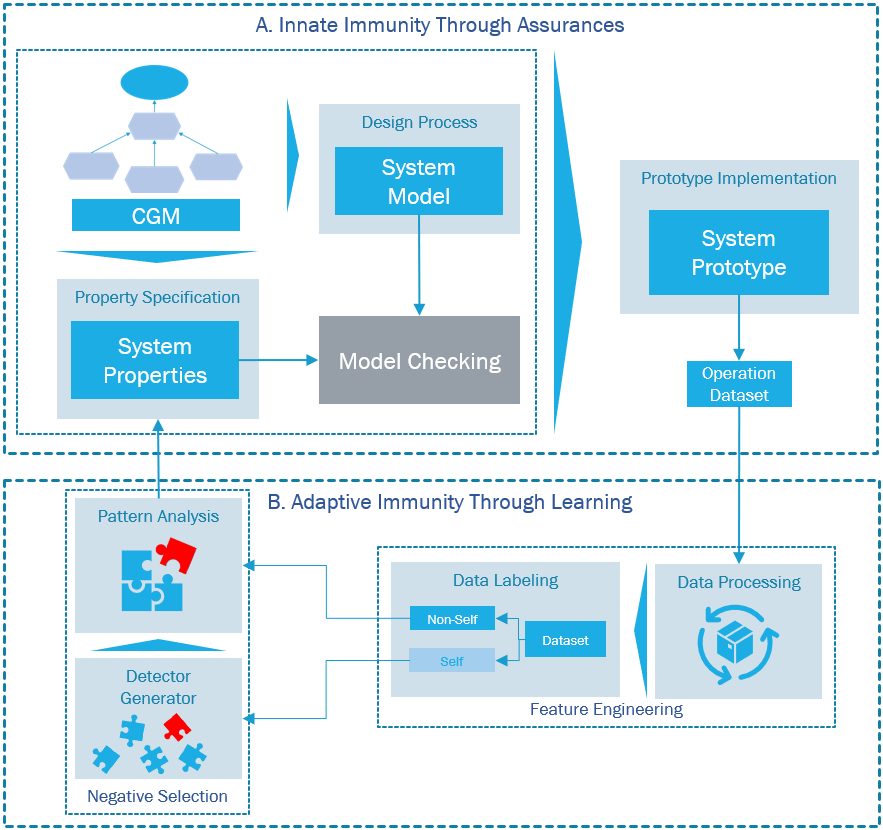
\includegraphics[width=0.999\textwidth, keepaspectratio]{img/overview_framework2.png}
	\caption{Overview of the proposed Methodology}
	\label{fig:FrameworkOverview}
\end{figure}

The second step happens right after the first one, and is performed individually for each property in the real-time property set. Initially, the operation data goes through a feature engineering process aiming at the labeling and characterization of the data traces that did not satisfy the particular property being examined. Next, the labeled data is analyzed, and  the Negative Selection Algorithm is used with the dataset. A collection of r-chunk detectors are produced as a result of this operation. These detectors, specialized in matching the property violation data, are carefully examined so that the patterns discovered can be comprehended. 

The outcome of this process is the identification of relevant context conditions that were not initially considered when designing the property. This information is, then, used to refine the property, and thus, enhance or create new observers. The enhanced observers trigger a new execution of the first step. The described steps go back and forth until no new relevant information is found. 


\section{Innate Immunity through Assurances}
% \section{From Goals to Properties}

The initial step of our approach has two primary objectives: the provision of assurances and the implementation of a prototype of the system being developed. An earlier project from our research lab, where the goal specification is mapped into models for real-time analysis, served as inspiration for both functions \cite{seams2018}.

\subsection{Model Checking}

This activity is related to the first goal. Providing assurances for the SAS happens by initially modeling the core architectural elements, along with their behavior, then by specifying a set of properties of interest, and finally, by conducting a model checking process in a verification tool like UPPAAL \cite{UPPAAL} to assert the system's correctness and the satisfiability of the properties.

First, the model is derived directly from the CGM, the input for this process. The intended behavior of the leaf-tasks are modeled as timed automata, according to the system architecture. The automata denote module templates, meaning that they might be reused if two instances share the same behavior. One of the possible modeling strategies is to use guard conditions and different locations in the model to portray the progression of the module's behavior, and thus, its life cycle. Hence, the progress and fulfillment of the CGM task's behavior may be depicted in the UPPAAL model as reachable states or locations, enabling the usage of reachability properties when verifying the correctness of the system.

Second, with the formalized model in hand, the next activity is to specify the set of properties that will be verified. In this sense, we might use the Autili et al. \cite{2015PropertySpecCatalog} property specification pattern catalog and framework (PSPFramework) to define the CGM properties. Property specification patterns have been effectively utilized to bypass the pragmatic hurdles of specification formalism, while still maintaining syntactic correctness and a true reflection of the system's intuition. This catalog comprises a list of property patterns, or categories, each relying on a set of structured English phrases, composed of terms that are denotable in temporal logics.

Each system property is specified in the PSPFramework in a top-down manner. A property category is first chosen from the catalog patterns list by the software developer, who then refines it with the specific scope and complementary attributes, like time or probability constraints. As a consequence, a sentence in structured English is created, which will then be mapped to an appropriate logic formalism. The mapping rule takes into account the property category and scope defined earlier to match a logic formula template from the catalog, which is written in a target language, like CSL or TCTL. Finally, the given time and probability constraints are inserted into the formula using an attribute assessment mechanism. The result is a formally expressed property, ready to be verified. In our work, the resultant property set will be written in Timed Computational Tree Logic (TCTL) \cite{1996TCTL}, since that is the language used by UPPAAL when verifying the formalized model's real-time features. 

Our work also leverages the use of the Observer Technique as an additional step towards providing evidence that the system behaves as expected. This approach is utilized in the checker to allow the verification of properties that go beyond simple reachability \cite{1998ReachabilityObs}. It consists of the translation of the TCTL formulas to finite-state automata that are added the model to be verified. These state machines are engineered to reach error states only when the observed property in the system model is violated \cite{1999Observers}. 
% Formally, the Observer can be defined as an automaton \(T_{\phi}\) that interacts with the system \(S\) in a way that none of the error states of \(T_{\phi}\) are reached if the property \(\phi\) is satisfied. 
The translation is performed by using an Observer Template catalog \cite{2022PSP} designed for model checking real-time systems in UPPAAL. Analogously to the property specification process, the property pattern and its corresponding scope are mapped to Observer UPPAAL template models in the catalog. As a result, each monitorable property will have a corresponding observer automata in the system model.

Finally, the generated formulas will be verified for reachability, safety or liveness in the modeled system, by a process called Model Checking. The TCTL model-checking problem is to determine for a particular timed automaton TA and TCTL formula \(\phi\) whether TA  \(\vDash \phi\) \cite{2008PrinciplesModelChecking}. In this work, a tool named UPPAAL \cite{UPPAAL} will be used to solve this problem by algorithmically assessing if the specified set of properties hold true for each possible state of the system model. If that is not the case, the model, the system specification and the system properties must be revised for a reverification.

\subsection{Prototype Implementation}

After assuring the correctness of the system through model checking, the second activity of this step is the implementation of a prototype for the system being developed. The major purpose is to replicate the system's behavior in order to generate reliable data for the context analysis process. The prototype operation dataset will be passed on to the next stage of our framework to convey the context discovery potential by means of artificial intelligence while still in the design phase.

The execution of the prototype can be easily related to the innate immunity, during the immunological response. The running simulation will be the first to face the contextual variability in the environment, just as the innate immunity is the first line of defense against the pathogens \cite{Kuby2019}. Inherited from the individual's progenitors, the nonspecific immunological mechanism is responsible for triggering the adaptive immunity by phagocyting the antigen and sending it to better enhance the lymphocytes. Similarly, our prototype is assured by "naive" observers, who may not be specific enough to account for all of the uncertainty in its surroundings. The observers are enhanced in the next step, by learning from the operation dataset, genereated by the simulation.

Having said that, the prototype is implemented by a simulation tool, based on the designed software architecture. Each module is build in a way to reflect the intended behavior of the system to be. The naive observers are also implemented so that the execution of the simulation may be monitored for the provision of assurances. In our work, we will use the Modelica language and the Open Modelica tool for this purpose.

The Modelica Language is a language used to design cyber-physical systems. It allows for the causal linking of modules that are regulated by mathematical equations \cite{Modelica}. It is a text-based language used to specify all components of a model, and to organize them into packages. In order to graphically edit and explore a Modelica model, as well as run model simulations and other analyses, a suitable Modelica simulation environment is required \cite{ModelicaSpecs}. The Open Modelica is a tool that fills in this gap by providing an open-source modeling and simulation environment for the Modelica language \cite{OpenModelica}. It is considered to be the most complete open-source modelica simulation tool \cite{OpenModelicaIM}.

With the prototype in place, many simulations with varying inputs, settings, and setups may be conducted to account for as much context variability as feasible. Each experiment will yield a dataset comprising the execution traces, resource usage, and context conditions at each stage of the execution. In the end, the generated datasets will be stored for the execution of the next step.


% \section{Enhancing Context Specification Through Learning}
\section{Adaptive Immunity Through Learning}

Our framework's next phase tries to improve context specification using learning approaches. It is performed for each monitorable TCTL property specified in the previous phases. The data created in the preceding stage, goes through a feature engineering process for reshaping and labeling the rows regarding the property satisfiability. Following that, the set of rows in which the property is met (self-set) is run through the Negative Selection Algorithm to build detectors for the complementary set (nonself-set). These detectors are evaluated in order to uncover novel context variability, which is then utilized to improve the observers.

% What do we mean by monitorable?
% https://github.com/lesunb/ais_bsn/wiki/Experiments
% https://github.com/hub-se/PSP-UPPAAL

We relate this step to the Adaptive Immunity mechanism that happens in our Biological Immune System, described in Section \ref{sec:bgBISOverview}, specially with the cellular immunity. T lymphocytes are used in this adaptive response, which are created in the bone marrow by a pseudo-random genetic rearrangement process and then developed in the Thymus by being tested against own cells \cite{AIS2014}. Similarly, our process generates randomly candidate strings that are tested for match against the operation dataset's self set, and, just as only T-cells that do not bind strongly with the self-cells are allowed to flow through the blood stream \cite{Kuby2019}, only the strings that do not match the self-set are used to enhance the observers later on.

This process can be further divided into two phases: the feature engineering phase, in which the operation dataset is reshaped and labeled, and the learning phase, where the Negative Selection algorithm generates nonself-detectors that are used to enhance the observers.
% \cite{seams2018}
% The data mining process enables us to isolate the component behaviors that need to be analyzed. The scope of analysis
% scales as we go up in the CGM treelike structure, that is, encompassing more elements in a database record and embracing all TCTL
% properties. By these means, the outcome of the data mining process
% provides evidence for the assurance check in our methodology

% As such, the enrichment of the goal model with causal relationship between context and the non-functional requirements fulfillment supports the anticipation of adaptation strategies and potentially mitigates runtime uncertainty 

% takes into account the structure of the Goal Model and the main concerns of the property to reshape the set and to label each row as a property violation or not.

\subsection{Feature Engineering}

This phase focuses on the shaping of the operation dataset in order to better adjust it to the learning algorithm. This is accomplished by first segmenting the data, then creating features to assist define individually a single segment, and lastly classifying the execution fragments as property violations (nonself) or not (self). 

The operation dataset is retrieved from Open Modelica as a collection of files, each of which is associated with a single simulation run in the previous step. A simulation file presents the data in a tabular manner, with the columns representing the values of the model's components, resources, signals and so on at every timestamp. The activities of segmentation, feature generation, and labeling are carried out for each individual file, and then concatenated in a resultant dataset.

Initially, the data is split based on the attributes or time constraints of the property being analyzed. For example, suppose the following property is being analyzed: "Whenever a sensor node has collected data, the central node will eventually process it". In this scenario, the attribute that indicates when the data has been collected will be used to segment the dataset. An execution segment will start when the collect signal is sent until right before the next signal. However, if the property is time-bound, the execution segment will begin when the collect signal is transmitted and last for the duration of the constraint. Figure \ref{fig:Segmentation} illustrates this process. The first column indicates the timestamp, whilst the others show the signals that were sent, with the thick blue box highlighting when the data was collected. On the one hand, the blue bracket alludes to the length of a property time-bounded by 2 seconds, while, on the other hand, the grey bracket indicates the length of the execution segment if only the signal is considered.

\begin{figure}[!h]
	\centering
	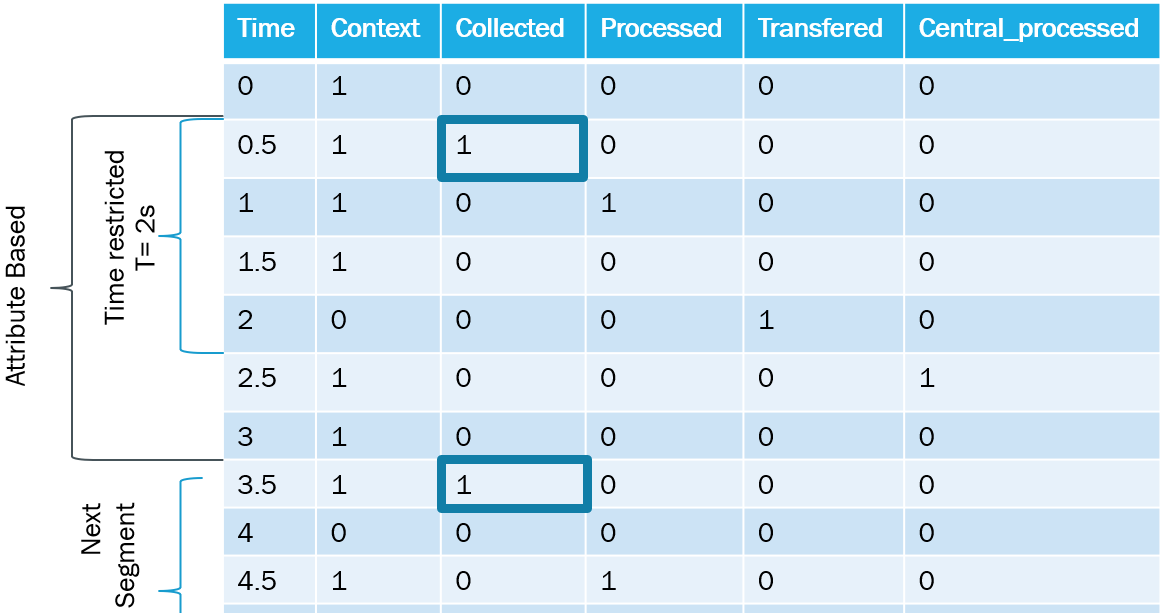
\includegraphics[width=0.999\textwidth, keepaspectratio]{img/Segmentation2.png}
	\caption{Segmentation based on attribute or on time restrictions}
	\label{fig:Segmentation}
\end{figure}

Next, new features will be derived to characterize the execution segment, resulting in a single row. For instance, in the abovementioned figure, it would be possible to create features for each signal, indicanting if the data was processed, transfered and if it was processed by the central node, or another that identifies if the context was true at all times. Continuous features could also be created, like one that stores the amount of time between processing and transfering the data, or how long it took for the central node to process the data, and so on. 

The quality and relevance of the features produced are essential for the development of the patterns that characterize the property violations, making this activity key to the effectiveness of our strategy. Additionally, it heavily depends on the domain knowledge of the software developer conducting the activity. The outcome is a new dataset, in which every row uniquely identifies and extracts the main features of an execution segment.

Finally, the classification phase will make use of the recently derived dataset. The rows will be examined in accordance with the TCTL property, and a label indicating whether the row describes a violation or can be regarded as a regular execution will be issued. Let again the property at hand be: "Whenever a sensor node has collected data, the central node will eventually process it". The execution segment should take into account whether the data was obtained and if the central node processed it. Both of these details may have been produced during the feature engineering stage and could be utilized in this instance for data labeling. If there is a boolean column with the value \textit{True} for a given segment, indicating that the data has been collected, and another boolean column with the value \textit{False}, indicating that the central node did not process the data, then it can be assumed that the given row, associated with the execution segment, violated the TCTL property.

\begin{figure}[!h]
	\centering
	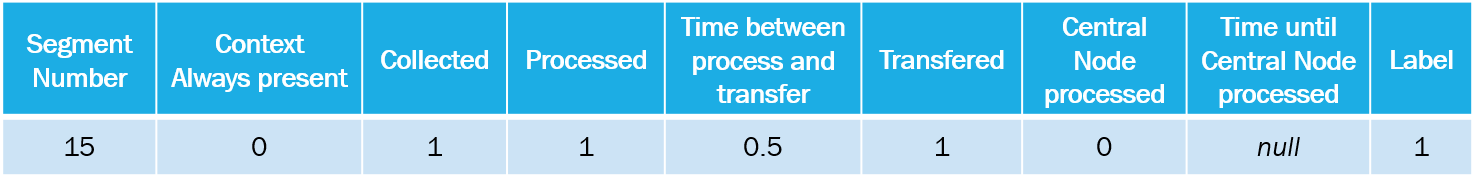
\includegraphics[width=0.999\textwidth, keepaspectratio]{img/FeatureEngResult.png}
	\caption{Example of a feature engineered execution segment}
	\label{fig:FeatureEngResult}
\end{figure}

Figure \ref{fig:FeatureEngResult} displays what would be the row associated with the time-restricted segment from Figure \ref{fig:Segmentation}. Since 2 seconds was not enough time for the central node to process the data, it was considered not done whithin the time window of th property. Hence, the column "Central Node processed" is zero, and "Time until Central Node processed" is \textit{null}, and therefore the row is labeled 1, meaning that this segment does violate the property.
% TODO: the observer signals are used as input for the labeling.

\subsection{Negative Selection Algorithm}

This final phase is the heart of the framework. It aims at using the Negative Selection Algorithm to try and find patterns in the nonself-set, in order to find new context variability that were not considered at first, and thus enhace the system's observers. This will be done in five steps. First, (i) the data obtained in the last phase will be analyzed so that the least relevant features may be discarded. Then, (ii) the remaining features will compose a string that will be used in the NSA. Next, (iii) the NSA will be performed and the nonself detectors will be generated and matured. Following that, (iv) the detector set will be thoroughly examined for the discovery of new context variability. Finally, (v) the information obtained will be used to refine both the system's TCTL properties and observers.

\subsubsection{i. Exploratory Data Analysis}

This initial step focuses on exploring the generated features to verify their relation with the property violation label, besides checking the integrity of the dataset. Another goal of this step is the selection of the features that will be used in the Negative Selection Algorithm.

Here, a series of dataset validations and verifications were conducted as part of a sanity check and preliminar analysis. First, the missing data are taken care of, and the required data types and ranges are adhered to the expected. The columns are then examined both singly and collectively to confirm their behavior. For instance, if data wasn't collected, it couldn't be processed. Thus, cases where the opposite happens are handled. This analysis also helps to decrease the number of features in the dataset by eliminating the columns that provide little or no information, based on their variance or the percentage of missing data.

Next, a correlation analysis takes place. Initially, the correlation matrix is computed, pairing the features and scoring their relationship. The features that are highly correlated, positively or negatively, indicate that the same information is provided and, thus, one of them is removed.

Finally, the features that will be used in the NSA are selected. Our work uses the binary version of the Negative Selection Algorithm, as described in Section \ref{sec:bgNSA}, meaning that only binary features can be used, at first. This being said, the boolean features are set apart and have their relation with the label measured. Since it does not matter much if the feature is positively or negatively correlated, only the absolute value is taken into account. Then, the features are sorted based on the strenght of the relationship and the ones that are below a certain threshold are discarded.

It is noteworthy to bring the reason why the columns were sorted. We shall employ the R-chunk as a matching rule in our work, which indicates that the detector candidate is often shorter than the string from the self-set. It is possible that relevant patterns are not seen if the columns are arranged randomly. This happens because the important bits might be positioned far apart and the chunk may be too short to consider all of them at once. The likelihood of this happening is reduced when the columns are arranged according to how strongly they relate to the label. Besides that, measuring the correlation allows us to filter out noisy features and, thus, enhance the result of the experiment.

The output of this step are the adjusted execution segment dataset and the ordered list of boolean features that will be used in the Negative Selection Algorithm. 

\subsubsection{ii. String formatting}

As detailed in Section \ref{sec:bgNSADistance}, the process of generation of detectors happens by measuring the similarity between the detector candidates and the dataset. In the binary version of the Negative Selection Algorithm, this assessment is usually performed by the means of a distance function, which compares the characters in two strings and returns a similarity score. 

In order to leverage the simplicity and efficiency of distance funcions in our work, this step will focus of formatting the dataset as binary strings. The input of this process will be the adjusted dataset created in the previous step, with only the boolean features selected after the correlation analysis, and ordered by the strength of the relationship with the label. The bits of the binary string for each row are made up of the contents of each column, with the leftmost bit coming from the column that is most correlated to the label, and the least significant bit comming from the column with the weakest relationship with the label.

\begin{figure}[!h]
	\centering
	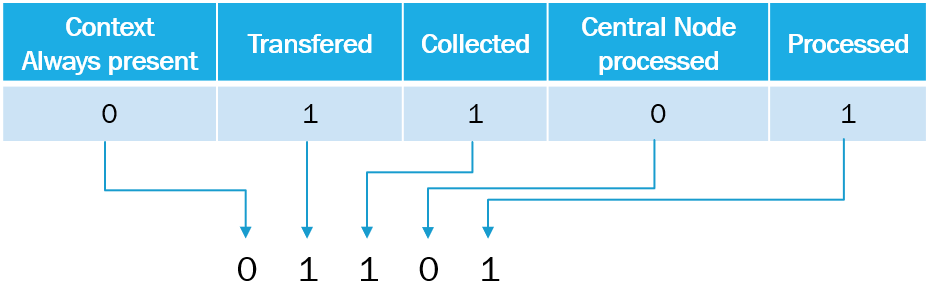
\includegraphics[width=0.7\textwidth, keepaspectratio]{img/stringFormatting.png}
	\caption{Formatting the dataset as binary strings}
	\label{fig:stringFormatting}
\end{figure}

Figure \ref{fig:stringFormatting} illustrates this process in the execution segment that is being used as an example throughout this section. To present the results of the correlation study from the previous phase, the columns have been sorted, the continuous features have been eliminated, and certain boolean columns have also been deleted.

\subsubsection{iii. NSA execution}

After gathering the data, preparing the dataset and formatting the strings, the dataset is ready to go through the Negative Selection Algorithm. This subsection will explain the implementation of the training phase of the algorithm, based on the theoretical background in Section \ref{sec:bgNSA}, that will be used in this work.

Our implementation of the NSA will meet the three requirements listed by Ji and Dasgupta \cite{RevisitingNSA2007} in order to be categorized as a Negative Selection Algorithm. It will make use only of the self-set (i) to randomly generate binary string detectors (ii) in order to identify the self-set counterpart (iii).

The use of only the self-set dataset is the first aspect to be taken into consideration. All rows with the label 1, meaning all rows that indicate a violation of the property of interest will be filtered out of the refined dataset, leaving just the self-set, or the set associated with the typical operation of the system. The idea is that the patterns of the nonself data will be derived from the examination of the self-set alone.

The second aspect considered in the NSA is the usage of detectors. Let \(X\) be a string from the self-set with size \(n\), such that \(X = x_1x_2x_3...x_n\). A candidate \(r\)-sized detector \(D\) is another binary string, with \(D = d_1d_2d_3...d_r\), with \(r \leq n\). The generate-and-test technique, which is further described in Section \ref{sec:bgNSADetectors}, will be used to construct the candidates. Simply put, as the name implies, this method generates random binary strings with a size of \(r\) to be compared with the strings in the self-set. 

The third and final aspect relates to the identification of the self-set counterpart. This will be done by comparing the candidate detectors to the set of self-strings, and discarding the ones that match. In our approach, we will use the R-Chunk distance function for the comparisons (refer to Section \ref{sec:bgNSADistance} for details). The candidates generated will be tested for each position \(p\), with \(0 \leq p \leq n-r\). If there's a match, the candidate is discarded. The remaining ones will be uniquely identified as \(t_{p, D}\) and stored for latter analysis. Therefore, the set of detectors will comprise only the candidates that did not match any self-set data.

% hyperparameters
The algorithm is greatly influenced by two hyperparameters: the size of the detector and the length of the detectors set. As mentioned before, too-short detectors could miss some significant patterns if the relevant features are placed far apart in the string. Long candidates, on the other hand, reduce the algorithm's efficiency since the number of potential strings that may be created at random rises exponentially with the chunk size. Additionally, lengthy detectors suffer from a loss of generalization since they have more fixed bits and, thus, detect less nonself data. The size of the detectors set also have a great impact on the final result, since sets with smaller lenghts may not cover the entire nonself-space and larger sets may increase the time needed to finish the execution. 

In this regard, we included a third hyperparameter to workaround the cases when the algorithm takes longer to converge. This parameter indicates the acceptable amount of failed attempts to add new candidates to the detectors set. If this value is reached, the algorithm will exit earlier.

The training of the algorithm will be performed as follows. First, the whole dataset will be split in two: one for the actual training and detector generation, and other for measuring the results and checking how well the detectors perform with unseen data. Second, the training set will have the nonself rows filtered out. Third, random strings of size \(r\) will be generated and tested against the self-strings in the training data in all possible positions. If there's a match, the detector candidate is discarded for that particular position. Otherwise, the string is stored along with the position in the detectors set. The third process is repeated until the length of the detectors set reaches a predefined size, or until no new detectors are added to the set after a fixed amount of attempts. Finally, the result of the learning phase is measured by using the detectors to predict property violations in the test set, which contains both self and nonself-data. The actual values are compared with the predicted values and the metrics of precision and recall are evaluated.

% TODO: Mention that only the training will be performed

\subsubsection{iv. Detector Analysis}

This step will be responsible for looking at the detectors that were created and understanding the patterns found. The R-Chunk detectors are identified in the set as \(t_{p, D}\), with \(p\) being the starting position and \(D\) the detector string of length \(r\). If step (ii) included mapping boolean features to bits in a string, here the mapping will be done in reverse. 

The detectors are sorted based on how many violations are matched. The most relevant ones go through this mapping to perform this analysis.

\begin{figure}[!h]
	\centering
	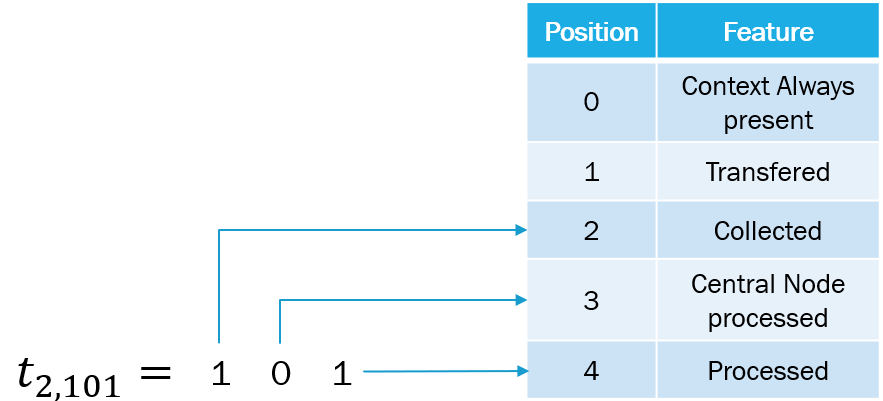
\includegraphics[width=0.7\textwidth, keepaspectratio]{img/detectoAnalysis.png}
	\caption{Mapping the Detectors to the features}
	\label{fig:detectoAnalysis}
\end{figure}

Figure \ref{fig:detectoAnalysis} shows how the mapping is done. The detector \(t_{2, 101}\) of size \(r = 3\) indicates a property violation pattern in position 2 with the values \(101\). By looking at the table with the corresponding features and positions, we can see that this pattern identifies the violations that happen when the data is collected, processed, but is not processed by the central node.  

One of the three features of the set may already account for context variability that was not yet considered. In this case, the next step could be performed right away. Otherwise, the remaining features that were not used in the generation of the detectors may come into play, like the weakly related booleans and the continuous variables that did not fit the algorithm. These features are analyzed specifically in the rows that were matched by the detector as an attempt to discover new hidden context combinations.


\subsubsection{v. Property Refinement}

Finally, after the new context variabiliy have been unveiled, the system's specification and properties are revisited. Initially, these contexts are properly elicited and returned to the Contextual Goal Model by a human analyst. Then, we iteratively map them to either existing or newly discovered system properties as well as to system model components. This means that, once we get to the final end of our approach, the updated CGM obtained as a result, is used as an input for a new execution of the whole methodology.

This stage is comparable to the conclusion of the BIS's adaptive immune response. In the human body, the lymphocytes that have undergone differentiation and maturation and have a high affinity for an antigen at hand are pumped via the bloodstream to the site of the inflammation. Whereas in our framework, the collection of NSA detectors triggers the development and improvement of observers, which are then put back into the system model to constantly check out for property violations while monitoring the newly revealed contexts.

% \section{Overview of the Proposed Methodology}
% TODO
